\documentclass[9pt]{beamer}
%\documentclass[handout]{beamer}

\usetheme{default}
\usecolortheme{dove}
\usefonttheme{professionalfonts}

\usepackage[utf8]{inputenc}
\usepackage{csquotes}
\usepackage[ngerman]{babel}
\usepackage[backend=biber,style=numeric,sorting=nyvt]{biblatex}
\usepackage{tikz}
\usetikzlibrary{arrows,shapes,shapes.geometric,positioning}
\usepackage[export]{adjustbox}
\usepackage{pifont}
\usepackage{epigraph}
\usepackage{graphbox}

\definecolor{MyGreen}{HTML}{80be08}
\definecolor{MyDarkGreen}{HTML}{004900}

%%%% BEGIN Custom Styling %%%%

\setbeamersize{text margin left=5mm,text margin right=5mm}

%\useinnertheme{rectangles}
%\useoutertheme{infolines}

\usepackage{fontspec}
\setsansfont{DeJaVuSans}

\setbeamercolor{itemize item}{fg=black}
\setbeamercolor{itemize subitem}{fg=black}
\setbeamercolor{itemize subsubitem}{fg=black}
\setbeamertemplate{itemize item}{\scriptsize\raise1.25pt\hbox{\textbullet}}
\setbeamertemplate{itemize subitem}{\tiny\raise1.5pt\hbox{\textbullet}}
\setbeamertemplate{itemize subsubitem}{\tiny\raise1.5pt\hbox{\textbullet}}
\setbeamertemplate{enumerate item}{\insertenumlabel.}
\setbeamertemplate{enumerate subitem}{\insertenumlabel.\insertsubenumlabel}
\setbeamertemplate{enumerate subsubitem}{%
  \insertenumlabel.\insertsubenumlabel.\insertsubsubenumlabel}
\setbeamertemplate{enumerate mini template}{\insertenumlabel}

% footer
\beamertemplatenavigationsymbolsempty

\setbeamertemplate{frametitle}{\textbf{\insertframetitle}\hfill}

\setbeamertemplate{footline}{%
  \begin{center}
    \color{MyGreen}
    \rule{0.93\textwidth}{0.05cm}
  \end{center}
  \vspace{-0.2cm}
  \hspace{0.5cm}%
  %\includegraphics[align=l, height=0.4cm]{../../images/project-logo.png}%
  \hfill%
  \usebeamercolor[fg]{page number in head/foot}%
  \usebeamerfont{page number in head/foot}%
  \selectfont\raisebox{0.15cm}{\insertframenumber\,/\,\inserttotalframenumber\kern1em}%
  \hfill%
  \color{MyGreen}%
  \textbf{\fontsize{8}{8}\selectfont\raisebox{0.15cm}{soundpaint.org}}%
  \hspace{0.45cm}{\ }
}

\newcommand{\clr}{MyDarkGreen}%

\setmainfont[
    Path           = /usr/share/fonts/truetype/freefont/,
    Extension      = .ttf,
    Ligatures      = TeX
]{FreeSans}

%%%% END Custom Styling %%%%

\newcommand{\cmark}{\ding{51}}%
\newcommand{\qmark}{\ding{51} / \ding{55}}%
\newcommand{\xmark}{\ding{55}}%
\newcommand{\imply}{$\Rightarrow$}

\title[Pico Simple Stupid Synth]{Pico Simple Stupid Synth}
\subtitle{Projektkurzvorstellung mit anschließender Diskussion}
\author{Jürgen Reuter}
\institute[\tt{soundpaint.org}]{\tt{soundpaint.org}}
\date[GPN22]{GPN 22\\30.~Mai 2024}

\AtBeginSection[] {
  \begin{frame}[t]{Überblick}
    \tableofcontents[currentsection]
  \end{frame}
}

\addbibresource{../../bib/gpn22.bib}

%\listfiles % DEBUG: show package versions in log

\begin{document}

\tikzstyle{every picture}+=[remember picture]
\everymath{\displaystyle}

\addtocounter{framenumber}{-1}

\begin{frame}[plain]
  \maketitle
\end{frame}

\begin{frame}[t]{Überblick}
  \tableofcontents
\end{frame}

\section{Ziele}

\begin{frame}[t]{Ziele}
  \begin{itemize}
  \item<2-> \color<2>{\clr} Pico als MIDI USB Device
  \item<3-> \color<3>{\clr} Proof-of-Concept MIDI Synth
  \item<4-> \color<4>{\clr} Schnelle, einfache Synthese
  \item<5-> \color<5>{\clr} Mindestens ca. 32-stimmig
  \item<6-> \color<6>{\clr} Audio-Ausgang via I²S oder analog
  \end{itemize}
\end{frame}

\begin{frame}[t]{Rechteckschwingungen}
  \begin{itemize}
  \item<2-> \color<2>{\clr} nur zwei Sample-Werte (abh.\ von Lautstärke)
  \item<3-> \color<3>{\clr} {\imply} bei Flanke das Delta zu Ausgangsumme addieren
  \end{itemize}
\end{frame}

\begin{frame}[fragile]{Audio-Ausgabe}
  \begin{itemize}
  \item<2-> \color<2>{\clr} I²S funktioniert
    \begin{itemize}
    \item<3-> \color<3>{\clr} Implementierung über Funktion in Pico SDK
    \item<4-> \color<4>{\clr} Ausgabe: GPIO 26 (BLCK), GPIO 27 (LRCLK), GPIO 28 (DATA)
    \item<5-> \color<5>{\clr} Analog-Wandlung über separaten Konverter
    \end{itemize}
  \item<6-> \color<6>{\clr} PWM funktioniert nicht
    \begin{itemize}
    \item<7-> \color<7>{\clr} im Code vorbereitet
    \item<8-> \color<8>{\clr} Stereo scheitert mutmaßlich an Bug in Pico SDK
    \item<9-> \color<9>{\clr} Außerdem Kollision in der Nutzung des 2.\ CPU Core
    \end{itemize}
  \end{itemize}
  \begin{center}
    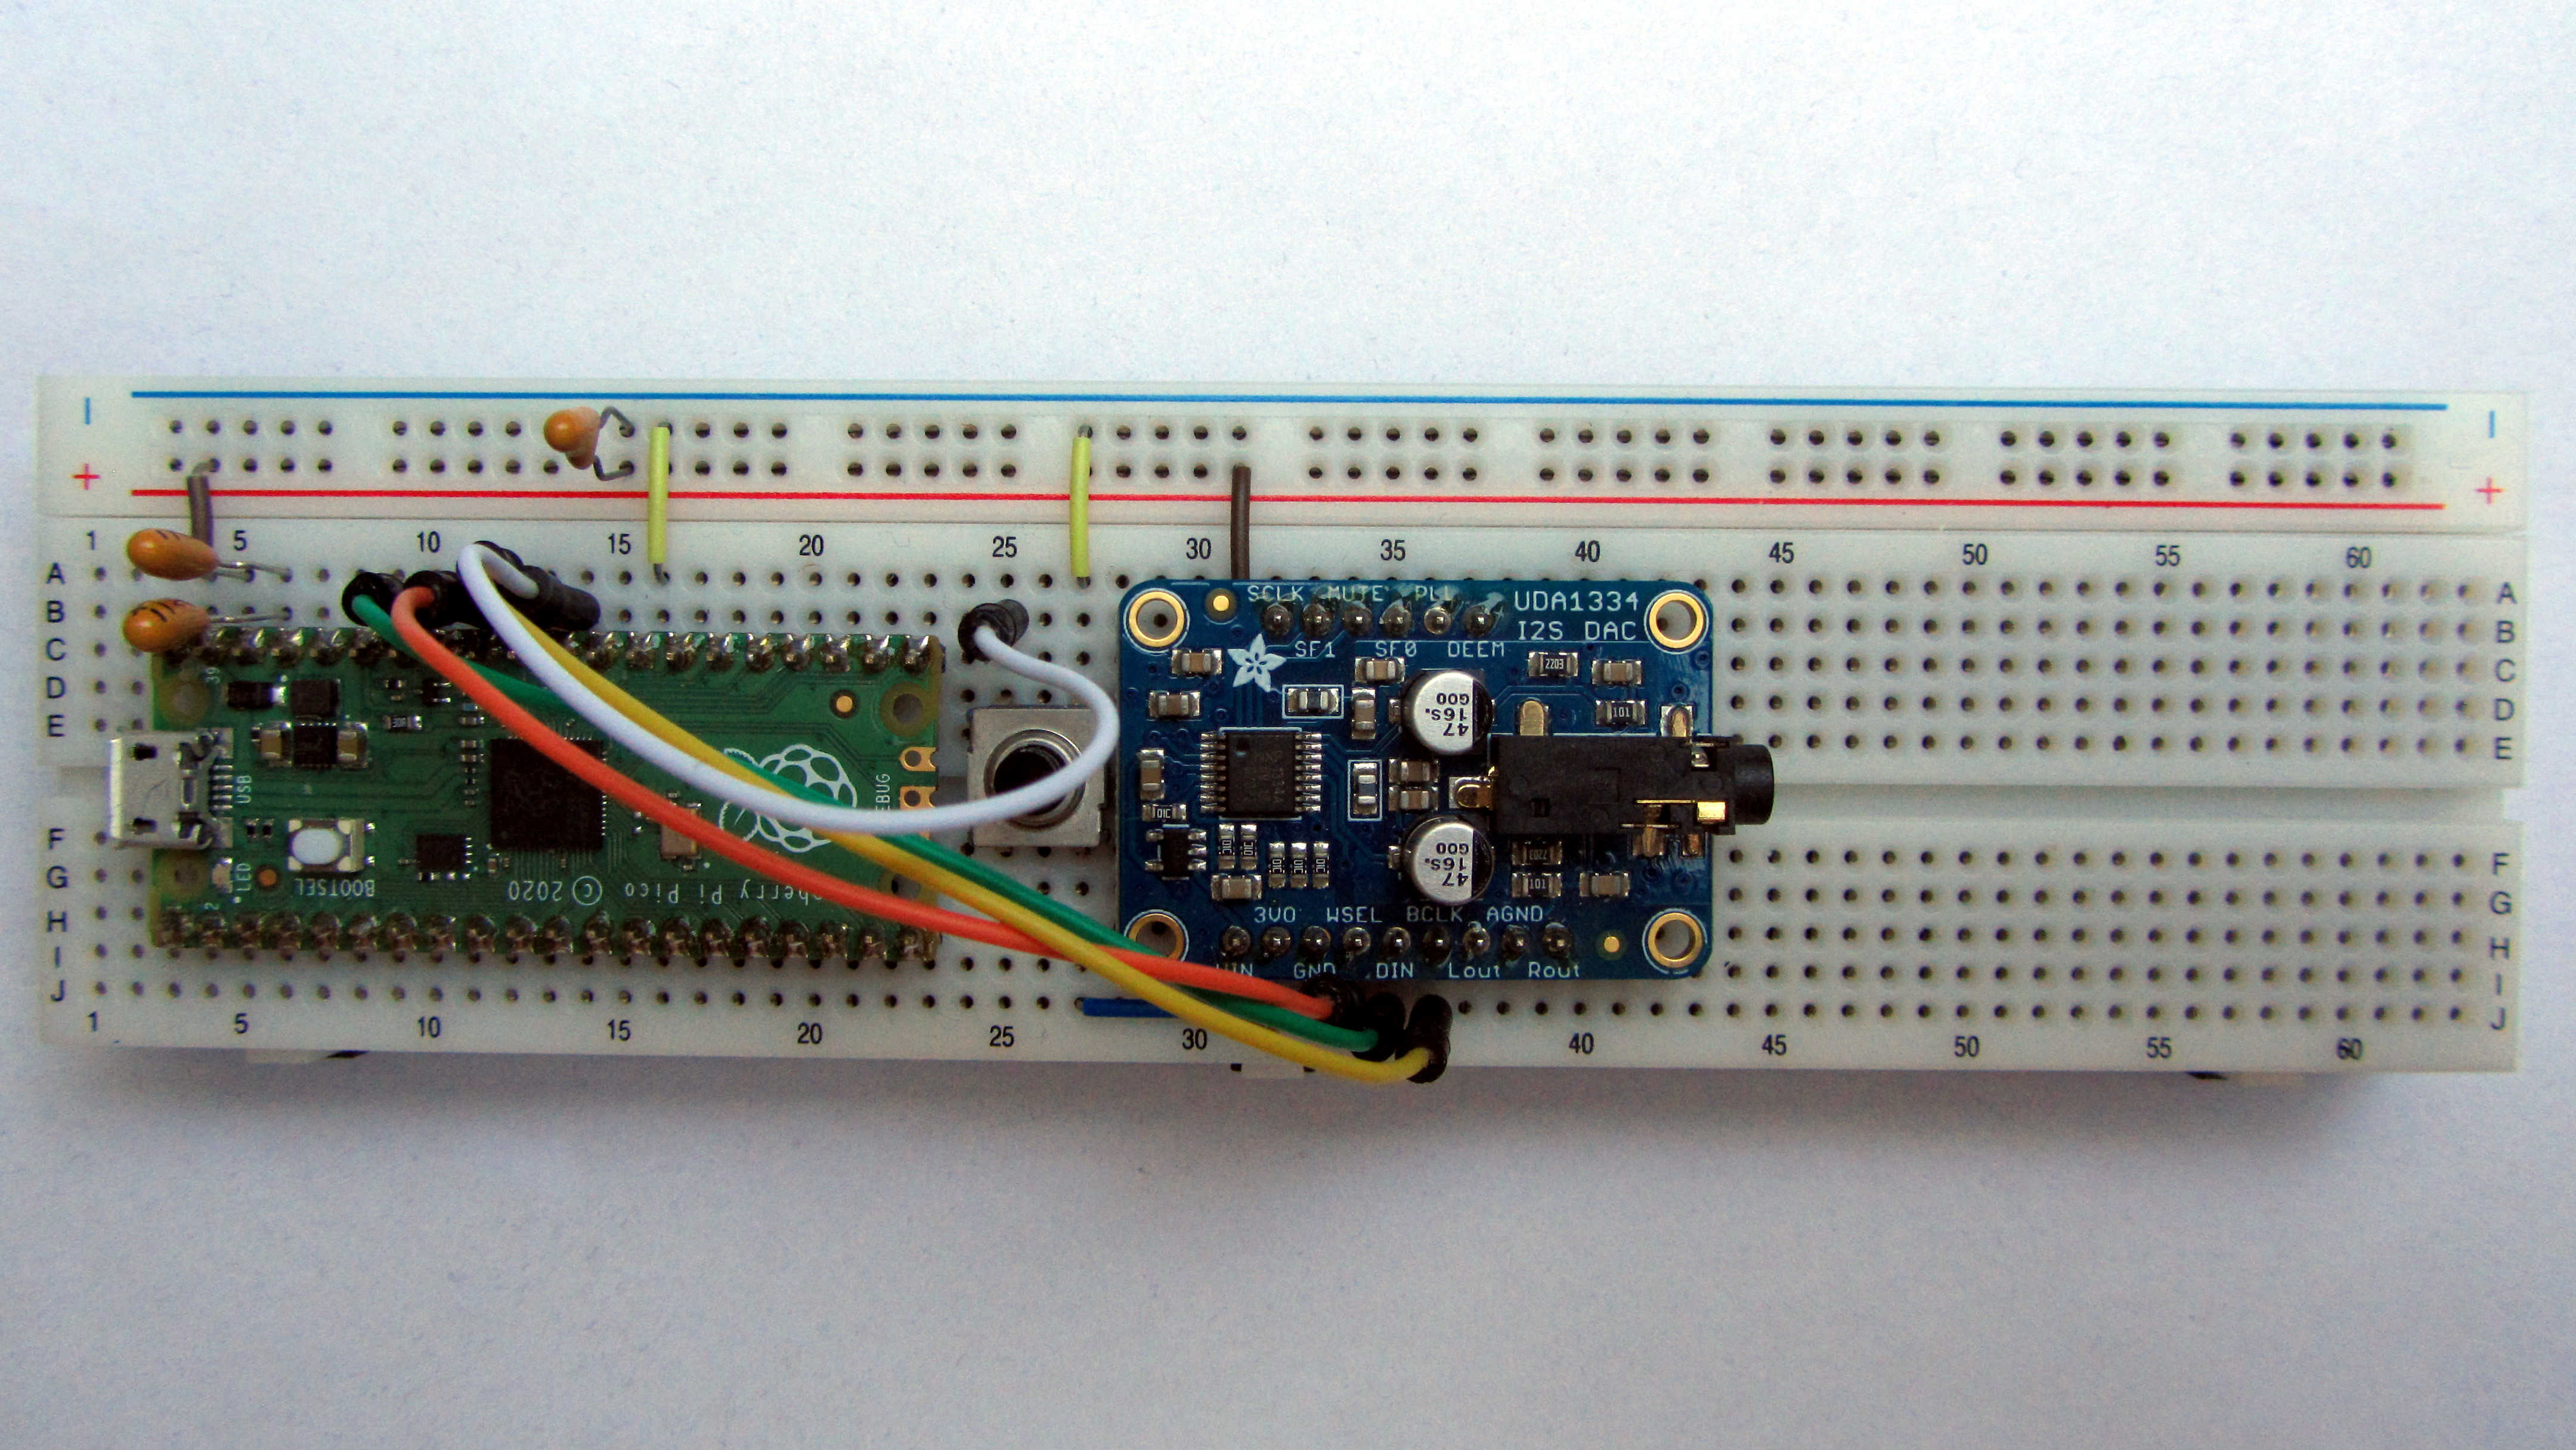
\includegraphics[width=0.75\textheight]{../../../../images/assembly-on-breadboard.jpg}
  \end{center}
\end{frame}

\begin{frame}[t]{Ergebnisse \& Ausblick}
  Ergebnisse
  \begin{itemize}
  \item<2-> \color<2>{\clr} gibt sich als MIDI Device aus
  \item<3-> \color<3>{\clr} bewältigt auch vielstimmige MIDI-Ströme
  \item<4-> \color<4>{\clr} Audio-Ausgang per I²S funktioniert
  \item<5-> \color<5>{\clr} analoger Audio-Ausgang funktioniert {\em noch nicht}
  \item<6-> \color<6>{\clr} sehr genaue und stabile Frequenzen dank Bresenham
  \item<7-> \color<7>{\clr} Proof-of-Concept als Basis für komplexere Designs
  \item<8-> \color<8>{\clr} Quellcode (GPL-2.0):
    \url{https://github.com/soundpaint/pico-simple-stupid-synth}
  \end{itemize}
  Ausblick
  \begin{itemize}
  \item<9-> \color<9>{\clr} voraussichtlich in Kürze multitimbrale Version
  \item<10-> \color<10>{\clr} später vielleicht deutlich komplexere
    Version auf Basis von Pico-Cluster
  \end{itemize}
\end{frame}

% bibliography
\section{Literaturverweise}

\begin{frame}[t,allowframebreaks]{Literaturverweise}
  \nocite{RaspberryPiLtd24a}
  \nocite{Reuter24a}
  \nocite{Wikipedia24a}
  \nocite{MIDIAssociation24a}
  \nocite{Thach24a}
  \printbibliography
\end{frame}

\section{Klang-Demonstration}

\begin{frame}[t]{Klang-Demonstration}
  {\em Trigger-Warning: Chiptune-artiger Sound mit hohen
    Frequenzanteilen (Rechteckschwingungen)}
\end{frame}

\begin{frame}[t]
  \begin{center}
    \Huge{Diskussion eröffnet!}
  \end{center}
\end{frame}

% backup slides

%\section{Anhänge}

%\section*{Schaltpläne}

%\begin{frame}[fragile]{Schematics}
%  \begin{center}
%    \includegraphics[width=0.75\textheight]{../schematics/synth.eps}
%  \end{center}
%\end{frame}

\end{document}

%  Local Variables:
%    coding:utf-8
%    mode:LaTeX
%  End:
